\chapter{Análisis del problema}
 
 Como todo software, esta aplicación se ha diseñado y desarrollado para cubrir unas necesidades muy bien definidas. En base a dicha premisa, podemos crear una descripción completa de los 
 actores, así como una lista de requisitos detallada con la que se cubran los objetivos previamente
 propuestos.

\section{Descripción de los actores}
Vamos a disponer de dos actores: el \textbf{usuario} y el \textbf{administrador}.\\

El \textbf{usuario} será el agente de policía que desee realizar cualquiera de las acciones
disponibles en la aplicación. Este actor no tiene por qué tener ninguna experiencia previa
con aplicaciones web, pero en este escenario se les ha formado con unas nociones básicas 
a modo de tutorial de cómo realizar todas las acciones posibles en la aplicación y las consecuencias
que tiene en el servidor. De esta manera, el usuario no tiene ningún problema interaccionando con la aplicación.\\

El \textbf{administrador} será la persona encargada de asegurar el correcto funcionamiento 
del software así como el encargado de la gestión de los datos de usuario y de la aplicación. Este
actor, por tanto, debe tener un alto conocimiento de las tecnologías con las que se ha construido
\textbf{Chief} para poder dar una rápida respuesta a los posibles problemas del usuario.

\section{Análisis de requisitos}

Los requisitos serán divididos en 3 tipos:

\begin{itemize}
   \item \textbf{Requisitos funcionales:} Son servicios que el sistema debe proporcionar, cómo
   debería responder a entradas concretas y como debe reaccionar el sistema en situaciones 
   particulares. En algunos casos, se puede especificar explícitamente qué no debe hacer el sistema.\cite{software-engineering}

   \item \textbf{Requisitos no funcionales:} Son requisitos que no tienen que estar directamente relacionado
   con el funcionamiento de la aplicación, sino más bien con el proceso del desarrollo.
   
   \item \textbf{Requisitos de información:} Estos requisitos están relacionados con la información 
   que se va a guardar en el sistema.
\end{itemize}

Para el siguiente punto se utilizarán las siguientes abreviaturas:\\
\renewcommand{\arraystretch}{1.5}
\begin{table}[H]
   \centering
   \label{tabla-abreviaturas}
   \begin{tabular}{|c|l|}
   \hline
   \textbf{Abreviatura} & \textbf{Significado} \\ \hline
   R.F X       & Para denotar el requisito funcional número \textit{X}.\\ \hline
   R.F X.Y     & Para denotar el subrequisito funcional número \textit{Y} de \textit{X}\\ \hline
   R.F X.Y.Z   & Para denotar el subrequisito funcional número \textit{Z} de \textit{Y}\\ \hline
   R.N.F X     & Para denotar el requisito no funcional número \textit{X}\\ \hline
   R.N.F X.Y   & Para denotar el subrequisito no funcional número \textit{Y} de \textit{X}\\ \hline
   R.N.F X.Y.Z & Para denotar el subrequisito no funcional número \textit{Z} de \textit{Y}\\ \hline
   R.I X       & Para denotar el requisito de información número \textit{X}\\ \hline
   R.I X.Y     & Para denotar el subrequisito de información número \textit{Y} de \textit{X}\\ \hline
   R.I X.Y.Z   & Para denotar el subrequisito de información número \textit{Z} de \textit{Y}\\ \hline
   \end{tabular}
   \caption{Tabla de abreviaturas para los tipos de requisitos.}
\end{table}


\subsection{Requisitos funcionales}
Los requisitos funcionales del desarrollo son los siguientes: 

\begin{itemize}
	
	\item \textbf{R.F 1}. Administración de los agentes.
	\begin{itemize}
		\item \textbf{R.F 1.1}. Registro de los agentes.
		\item \textbf{R.F 1.2}. Acceso de los agentes.
		\item \textbf{R.F 1.2}. Cerrar sesión.
	\end{itemize}

	\item \textbf{R.F 2}. Administración de turnos.
	\begin{itemize}
		\item \textbf{R.F 2.1}. Crear un documento de turno.
		\item \textbf{R.F 2.2}. Crear una nueva incidencia.
		\item \textbf{R.F 2.3}. Finalizar un parte de servicio.
	\end{itemize}

	\item \textbf{R.F 3}. Creación de ordenanzas.
	\begin{itemize}
		\item \textbf{R.F 3.1}. Crear una ordenanza de limpieza.
		\item \textbf{R.F 3.2}. Crear una ordenanza de ruidos.
		\begin{itemize}
			\item \textbf{R.F 3.2.1}. Crear un acta de molestias de ruidos en la vía pública.
			\item \textbf{R.F 3.2.2}. Crear un acta de molestias de ruidos en domicilio.
			\item \textbf{R.F 3.2.3}. Crear un acta de molestias de ruidos en local.
			\item \textbf{R.F 3.2.4}. Crear un acta de medición de ruidos.
		\end{itemize}
		\item \textbf{R.F 3.3}. Crear una ordenanza de obras.
		\begin{itemize}
			\item \textbf{R.F 3.3.1}. Crear un acta inspección de obras.
		\end{itemize}
		\item \textbf{R.F 3.4}. Crear una ordenanza de residuos.
		\begin{itemize}
			\item \textbf{R.F 3.3.1}. Crear un acta hallazgo de residuos.
		\end{itemize}
	\end{itemize}

	\item \textbf{R.F 4}. Creación de partes de accidentes.
	\begin{itemize}
		\item \textbf{R.F 4.1}. Crear parte de accidente de 2 vehículos.
		\item \textbf{R.F 4.2}. Crear parte de accidente de 3 vehículos.
	\end{itemize}

	\item \textbf{R.F 5}. Administrar croquis.
	\begin{itemize}
		\item \textbf{R.F 5.1}. Crear un croquis.
		\item \textbf{R.F 5.2}. Enviar un croquis.
	\end{itemize}


\end{itemize}

\subsection{Requisitos no funcionales}
Los requisitos no funcionales del desarrollo son los siguientes: 

\begin{itemize}
	\item \textbf{R.N.F 1}. La aplicación se aprovisionará automáticamente.
	\item \textbf{R.N.F 2}. Se utilizarán solamente módulos NPM como dependencias del sistema. 
	\item \textbf{R.N.F 3}. Se desplegará en una máquina virtual en un entorno controlado.
	\item \textbf{R.N.F 5}. Se creará la estructura de directorios necesaria de manera automática. 
	\item \textbf{R.N.F 5}. Para utilizar el sistema de documentos se deberán proporcionar las plantillas.
	\item \textbf{R.N.F 6}. La creación de las máquinas virtuales se realizará automáticamente.
	\item \textbf{R.N.F 7}. La base de datos se creará sin necesidad de administrarla.
\end{itemize}

\subsection{Requisitos de información}
La base de datos de la aplicación almacenará los mínimos datos necesarios, De este modo conseguimos aumentar la seguridad global del sistema:

\begin{itemize}
	\item \textbf{R.I 1}. Datos de usuario.
	\begin{itemize}
		\item Información necesaria para poder identificar a los usuarios del sistema.
		\item ID interno, usuario, contraseña, email, nombre y apellidos.
	\end{itemize}

	\item \textbf{R.I 2}. Datos de incidencias.
	\begin{itemize}
		\item Información necesaria para poder definir correctamente una incidencia dentro de un parte de servicio.
		\item Número identificador, fecha, hora, dependencia, central, número de agente, hecho y actuación.
	\end{itemize}
\end{itemize}

\section{Análisis de las soluciones}

Como en el desarrollo de cualquier software, no existe una solución única. Por tanto, se deben analizar las
distintas tecnologías que hay en el mercado para garantizar que la solución propuesta es la más adecuada para
los problemas que se plantean.

\subsection{Back-end}

\subsubsection{Elección del servidor} 
A la hora de crear una aplicación web, tenemos un amplio abanicos de posibilidades sobre las que crear nuestro servidor. Aunque, en este caso
en concreto, se le ha añadido una restricción y es que el servidor debe ser \textit{open source}. Para obtener
una idea global se puede observar el siguiente gráfico comparativo del uso de distintas tecnologías en los servidores web actuales:

\begin{figure}[H]
	\centering
	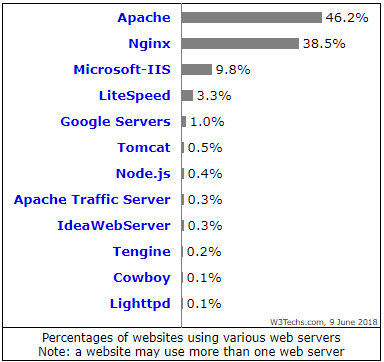
\includegraphics[scale=0.8]{imagenes/web-servers-comparison.png}
	\caption{Comparativa de servidores web.\cite{web-server-usage} \label{fig:figura2}}
\end{figure}

Es inmediato captar la superioridad de Apache\cite{apache} en esta gráfica. Esto se debe, principalmente, a que su lanzamiento 
oficial fue en el año 1996. En esta época no tuvo ningún rival y por tanto se posicionó el primero en el mercado, 
persistiendo aún hoy en día en un gran número de equipos.\\

Sin embargo, en esta lista de servidores todos siguen el esquema tradicional en el que cada petición es atendida 
por una hebra del sistema. En la situación actual del desarrollo web, se está optando por una nueva metodología. La programación
asíncrona orientada a eventos. En este tipo de arquitecturas se consigue un mejor rendimiento con un menor coste 
de recursos debido a la escalabilidad que poseen. \\

En la siguiente imagen podemos ver la diferencia entre un sistema convencional y el utilizado por Node.js\cite{nodejs}.

\begin{figure}[H]
	\centering
	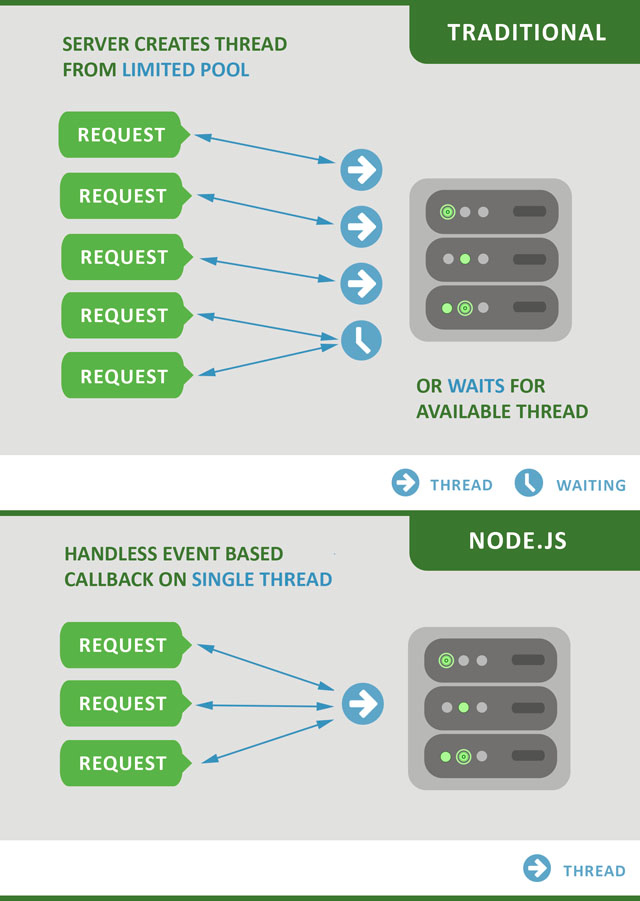
\includegraphics[scale=0.5]{imagenes/traditional-vs-nodejs.jpg}
	\caption{Sistema convencional vs Node\cite{image-node} \label{fig:figura3}}
\end{figure}

El único servidor web que presenta este tipo de arquitectura es Node.js y es por ello por lo que está
ganando una gran popularidad a medida que pasa el tiempo. Su porcentaje de uso aún es bajo debido a que es una tecnología 
bastante nueva y que está ganando atención en los últimos años, como podemos comprobar en el siguiente gráfico
de tendencia:

\begin{figure}[H]
	\centering
	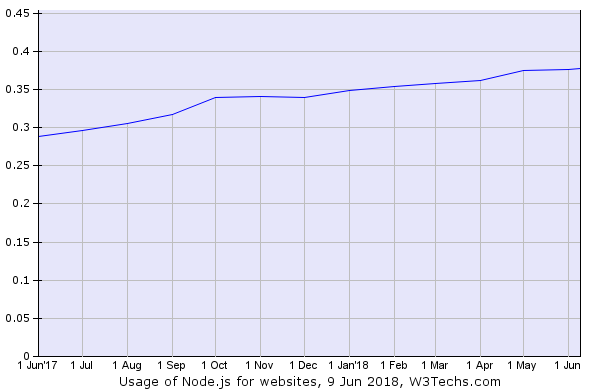
\includegraphics[scale=0.65]{imagenes/nodejs-trend.png}
	\caption{Gráfico de tendencia de Node.js \cite{nodejs-trend} \label{fig:figura4}}
\end{figure}

Además, Node.js dispone de \textit{npm}\cite{npm}, que es la herramienta de gestión de paquetes por defecto de Node. Este
gestor de paquetes fue creado con la intención de ayudar a los desarrolladores de JavaScript  de todo el mundo a compartir y utilizar
módulos de código creados por la comunidad. Lo más destacable de
de este proyecto es la acogida que ha tenido, adquiriendo decenas de miles de usuarios que, además, se involucran
activamente en el desarrollo. De esta manera consiguen una mejora constante del software. Por tanto, se ha logrado conseguir
un gran número de paquetes y hace que el desarrollo con Node sea más liviano, rápido y eficiente. Podemos utilizar paquetes que 
ha desarrollado la comunidad de una manera muy sencilla, ahorrando costes en el tiempo del desarrollo.


\subsubsection{Elección de la base de datos}

En este apartado tenemos dos grandes corrientes: bases de datos relacionales o no relacionales. Dicho de otra manera,
bases de datos \textbf{SQL} o \textbf{NoSQL}. Ambas son opciones completamente válidas pero tienen sus diferencias y serán analizadas a continuación.\\

Las bases de datos SQL utilizan un lenguaje de consulta estructurada (\textit{\textbf{S}tructured \textbf{Q}uery \textbf{L}anguage}) para manipular
y definir los datos. Este tipo de consulta es una de las más usadas y es muy útil para realizar consultas complejas. 
Pero, por otro lado, es muy restrictiva ya que te exige definir la estructura de los datos que se van a almacenar \textbf{antes} 
de realizar cualquier operación y comenzar a trabajar. Esto impacta de manera directa con el tiempo que se debe dedicar a 
la preparación y al planteamiento de los datos que vamos a utilizar y guardar, ya que modificar dicha estructura posteriormente
puede ser realmente costoso y provocar una desestabilización completa de la base de datos.\\

Por otra parte, las bases de datos NoSQL, usualmente llamados \textbf{no sólo SQL}, para destacar que también pueden soportar consultas de tipo SQL. Poseen un esquema dinámico para gestionar los datos no estructurados. Este hecho se puede traducir directamente en las siguientes características:

\begin{itemize}
	\item Se pueden añadir datos sin haber definido previamente su estructura.
	\item Los campos puede cambiar con el tiempo, incluso aparecer o desaparecer.
	\item Cada documento puede tener su propia estructura.
\end{itemize}

Una vez presentadas ambas opciones, podemos comparar sus características y optar por la que mejor se adapte a nuestro producto.

\renewcommand{\arraystretch}{2}
\begin{table}[H]
	\centering
	\resizebox{\textwidth}{!}{%
	\begin{tabular}{@{}ccc@{}}
		\toprule
		\rowcolor[HTML]{ECF4FF} 
		& \textbf{SQL}                                                                                                     & \textbf{NoSQL}                                                                                                               \\
		\cellcolor[HTML]{ECF4FF}\textbf{Datos}        & Estructurados en tablas                                                                                          & Estructuradas en documentos                                                                                         \\
		\rowcolor[HTML]{EFEFEF} 
		\cellcolor[HTML]{ECF4FF}\textbf{Esquema}      & Estático                                                                                                         & Dinámico o flexible                                                                                                          \\
		\cellcolor[HTML]{ECF4FF}\textbf{Escalablidad} & Vertical                                                                                                         & Horizontal                                                                                                                   \\
		\rowcolor[HTML]{EFEFEF} 
		\cellcolor[HTML]{ECF4FF}\textbf{OLTP}         & Recomendada para este tipo de sistemas                                                                           & Menos utilizadas en estos sistemas                                                                                           \\
		\cellcolor[HTML]{ECF4FF}\textbf{Consistencia} & ACID\cite{acid}                                                                                                  & Teorema  CAP\cite{cap}                                                                                                                  \\
		\rowcolor[HTML]{EFEFEF} 
		\cellcolor[HTML]{ECF4FF}\textbf{Rendimiento}  & \begin{tabular}[c]{@{}l@{}}Inversamente proporcional al volumen \\ de datos almacenado actualmente.\end{tabular} & \begin{tabular}[c]{@{}l@{}}Alto y con posibilidad de mejora a costa \\ de reducir la consistencia de los datos.\end{tabular}
	\end{tabular}}
	\caption{Bases de datos SQL vs NoSQL}
\end{table}

Una vez comparadas ambas, podemos comprobar que las bases de datos SQL son especialmente útiles en sistemas robustos, muy bien definidos desde el principio
en el que no se esperan cambios drásticos en la estructura de sus datos. Mientras que las bases de datos NoSQL son útiles cuando buscamos un sistema de se adapte en función de las necesidades del usuario o del propio desarrollo y que además no suponga grandes costes cuando se decida aumentar la escalabilidad del sistema.\\

Por otro lado, también se debe tener en cuenta la \textbf{consistencia} de los datos. Como hemos comprobado, las bases de datos SQL garantizan la consistencia de sus datos por diseño, mientras que en el otro tipo, no se garantiza de un modo tan fiable. Por ello, las bases NoSQL se utilizan cuando manejamos un alto volumen de datos ya que es necesario adaptarse a esta cantidad de tráfico. 


\subsection{Front-end}

Debido a que se a priorizado el desarrollo del \textit{back-end} y su correcto funcionamiento, en esta parte se han optado por tecnologías ya conocidas y utilizadas durante el transcurso del grado.

\subsubsection{Elección del motor de plantillas}

Se ha elegido Pug\cite{pug} ya que es un motor de plantillas de alto rendimiento. Este motor de plantillas era conocido anteriormente como Jade\cite{jade}, pero al tiempo
los desarrolladores se dieron cuenta de que esa marca ya estaba registrada y por tanto tuvieron que cambiar el nombre al proyecto. Cabe destacar,
que debido a la popularidad de Jade, se sigue utilizando en algunas webs pero el paquete ya no cuenta con el soporte oficial y todas las actualizaciones se lanzarán bajo el nuevo nombre. \\

La principal ventaja de este motor de plantillas es su mínima curva de aprendizaje. Esto se debe a que la sintaxis que utiliza es extremadamente sencilla y puede permitir a cualquier usuario crear páginas web en HTML de una manera muy intuitiva como podemos comprobar en el siguiente ejemplo:

\begin{figure}[H]
	\centering
	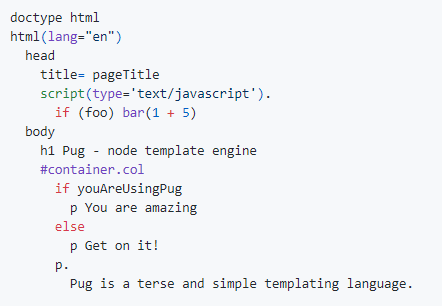
\includegraphics[scale=0.85]{imagenes/pug-example.png}
	\caption{Página de ejemplo escrita en Pug. \label{fig:figura8}}
\end{figure}

Este código será transformado directamente en el siguiente, ya interpretable por el navegador.

\begin{figure}[H]
	\centering
	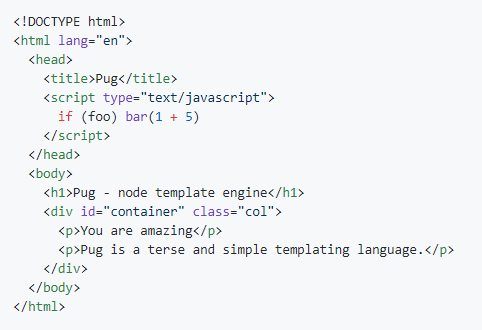
\includegraphics[scale=0.85]{imagenes/pug-rendered.png}
	\caption{Resultado del código ya interpretado. \label{fig:figura9}}
\end{figure}


\subsubsection{Elección del framework CSS}

En \textbf{Chief} se persigue conseguir una interfaz sencilla para que sea lo más simple e intuitiva posible de cara al usuario. De esta manera, la curva de aprendizaje
para utilizar el producto sería mínima. Por tanto, se ha optado por elegir Bootstrap.\\

Boostrap\cite{bootstrap} es la herramienta \textit{open-source} para desarrollo web por excelencia. Es uno de los proyectos libres más populares y utilizado por toda la comunidad.
Fue creado por un trabajador de Twitter a mediados del 2010. Antes de ser el proyecto libre que es ahora, era privado ya que Twitter poseía los derechos sobre el mismo.
Pero todo cambió cuando Twitter celebró su primera Hack Week\cite{hack-week} y vieron la acogida del proyecto por parte de toda la comunidad de desarrolladores. Siguió en desarrollo
durante un año después de dicho evento y, finalmente, se publicó la primera versión del \textit{framework} tan conocido a día de hoy.\\

Debido a su simpleza a la hora de ser utilizado y a lo sencilla que es su sintaxis, se pueden crear páginas web completamente adaptables de una manera muy rápida e intuitiva. Además, al ser tan conocido en la comunidad hay una gran cantidad de tutoriales en los que se enseña a utilizarlo desde 0.

\newpage

\section{Solución propuesta}

En base al análisis anterior, se ha decidido utilizar como dato base para la aplicación JSON\cite{json}.\\

El motivo principal es que debido a las características del desarrollo a realizar y los requerimientos del sistema,
una base de datos \textbf{NoSQL} era la opción idónea para este software. Esto es debido a que como hemos comprobado,
es una base de datos muy flexible, que permite la incorporación de nuevos campos sin provocar grandes problemas en 
la base de datos ni desestructurarla por completo.\\

Además, dado que el objetivo del desarrollo es conseguir un prototipo funcional, con el tiempo se le podrán añadir
nuevas funcionalidades, nuevos tipos de usuarios, nuevos campos a las incidencias... Por tanto, para garantizar 
la consistencia del sistema en un futuro se ha optado por este tipo de base de datos.\\

Finalmente, después de un estudio completo de las tecnologías más usadas actualmente en aplicaciones con unas características similares a \textbf{Chief}, la solución al problema inicial se ha conseguido 
mediante el uso de las siguientes tecnologías.

\subsection{Node.js}

Node.js es un entorno de ejecución para JavaScript construido con el motor de JavaScript
V8 de Chrome. En este proyecto se ha utilizado para elaborar el servidor de la aplicación.\\

Node.js tiene una característica que lo diferencia del resto de posibilidades para implementar 
el servidor, como comentamos anteriormente, y es que utiliza un modelo de operaciones E/S sin bloqueo y orientado a eventos 
\textbf{asícronos}. Esto nos ofrece la posibilidad de que cuando se detecte una conexión se atienda
pero el resto del tiempo estará inactivo, no malgastando potencia de computo ni energía. Con este nuevo modelo conseguimos servidores altamente 
escalables de una manera muy sencilla, rápida y eficiente.\\

\begin{figure}[H]
	\centering
	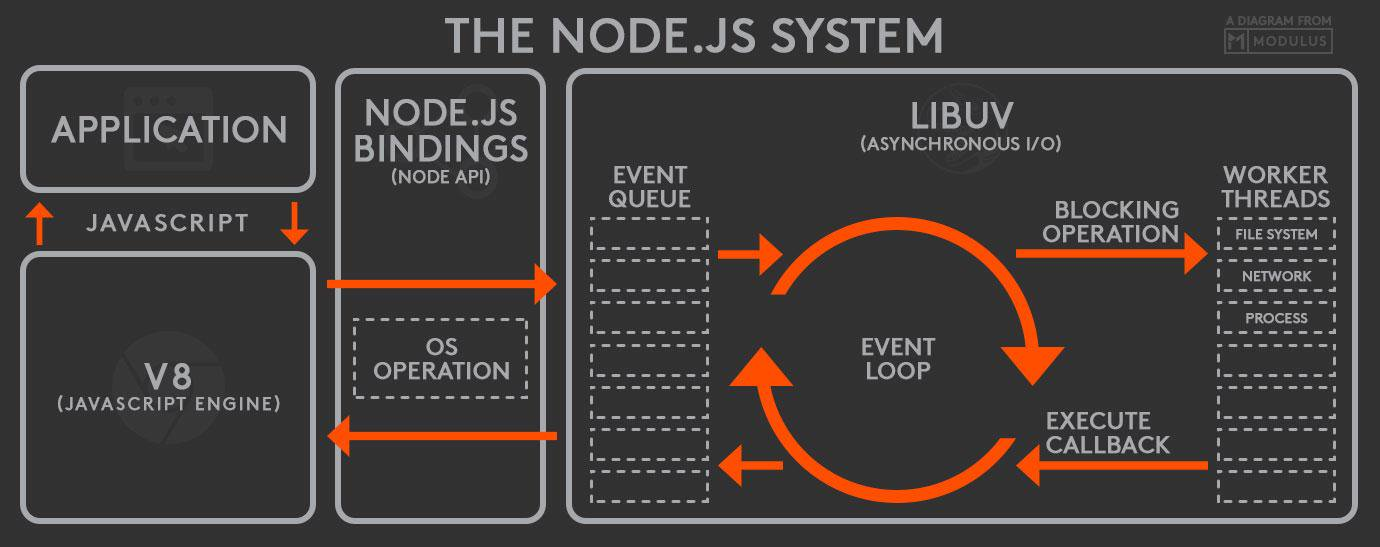
\includegraphics[scale=0.25]{imagenes/nodejs_system.jpg}
	\caption{Arquitectura de Nodejs\cite{image-node-arch} \label{fig:figura1}}
\end{figure}

Este diseño contrasta directamente con el modelo de concurrencia más común hoy en 
día en el que se usan hilos del Sistema Operativo para resolver peticiones. Las operaciones en red basadas en este modelo son relativamente ineficientes además de complejas en su uso. Cabe mencionar que, aunque Node.js 
no utilice hilos del Sistema Operativo del mismo modo que los servidores clásicos, no implica que no podamos aprovechar los múltiples núcleos de nuestro sistema.\\

Otro punto a favor de Node.js es que no tendremos que preocuparnos por la posibilidad de un 
bloqueo en el proceso debido a que no existe dicha posibilidad por la naturaleza de dicha 
tecnología, la cual, como se ha comprobado, está basada en un bucle de eventos.

\subsection{MongoDB}

MongoDB es un sistema de base de datos multiplataforma y orientado a documentos de esquema libre.
Esto quiere decir que cada entrada puede tener un esquema de datos diferente al anterior, por
lo que podemos tener entradas que difieran en el número de atributos entre sí.\\

Debido a esta característica los datos no son guardados en registros, como en las bases SQL, 
sino que se guardan en documentos. Estos archivos son del tipo BSON, que es una representación
binaria de los archivos JSON.\\

Esta tecnología ha sido escrita en C++, por lo que está en contacto con el \textit{bare metal}. Esto
último es realmente importante ya que le permite optimizar los recursos y acceder a ellos de una 
manera extremadamente eficiente, con lo que consigue una velocidad muy alta en todas sus operaciones.\\

Cabe mencionar que MongoDB es una plataforma completamente distribuida, lo que nos proporciona 
un nuevo nivel de escalabilidad y disponibilidad. Esto quiere decir que a medida que nuestro desarrollo
crezca tanto en volumen de datos como en rendimiento MongoDB se escala automáticamente sin tiempos
de caída y sin cambios en nuestra aplicación.\\

Mediante la utilización del paquete de \textit{npm} llamado \textit{Mongoose}\cite{mongoose}, la integración de MongoDB
con Node.js se realiza de una manera muy sencilla y rápida, por lo que la utilización de este módulo
cuando trabajamos con ambas tecnologías es ideal. En la siguiente imagen se define el flujo de datos
estándar cuando trabajamos con este esquema:

\begin{figure}[H]
	\centering
	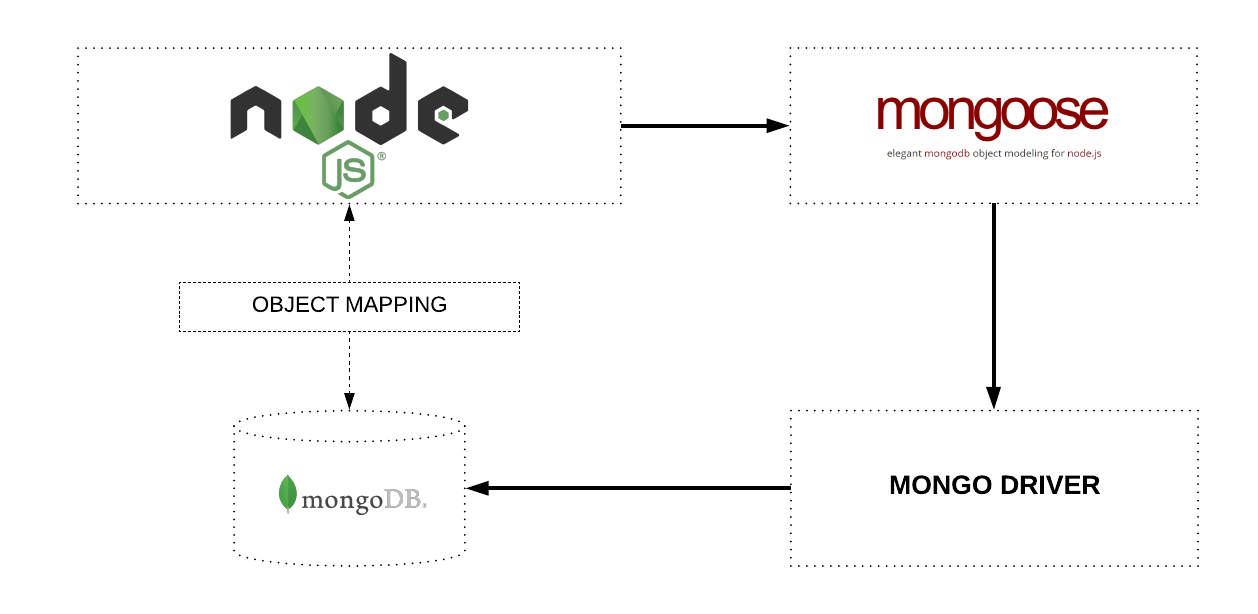
\includegraphics[scale=0.28]{imagenes/node-mongo.png}
	\caption{Flujo de datos con Node.js, Mongoose y MongoDB.\cite{image-mongoose} \label{fig:figura5}}
\end{figure}


Por último, cabe mencionar que la licencia de esta tecnología es GNU AGPL 3.0\cite{agpl}, por lo que se trata de un software con licencia
libre.


% gráficas de uso frente al resto de bbdd

\subsection{Vagrant}

Vagrant\cite{vagrant} es una herramienta creada para construir y administrar entornos de máquinas virtuales de una 
manera sencilla. Debido a que está diseñado para ser sencillo de utilizar y a que se centra en 
la automatización hace que utilicemos el menor tiempo posible en la preparación del entorno virtual
que necesitamos para comenzar a trabajar.\\

Nos proporciona un entorno muy rápido y simple de configurar, reproducible y portable utilizando
tecnología puntera en el sector de la virtualización como puede ser VirtualBox, VMWare, AWS, Docker...\\

Una enorme ventaja que aporta Vagrant al desarrollo es la posibilidad de aislar toda la configuración
del entorno y todas sus dependencias. Además, no hay que cambiarlas herramientas de trabajo usuales, pues realmente se sigue trabajando en la misma máquina. 
De esta manera se consigue un desarrollo más eficiente y con mínimas pérdidas de tiempo, garantizando 
de manera directa una eficiencia en la gestión de los recursos humanos empleados.\\

En la siguiente imagen se puede ver como funciona el flujo de trabajo utilizando esta herramienta:

\begin{figure}[H]
	\centering
	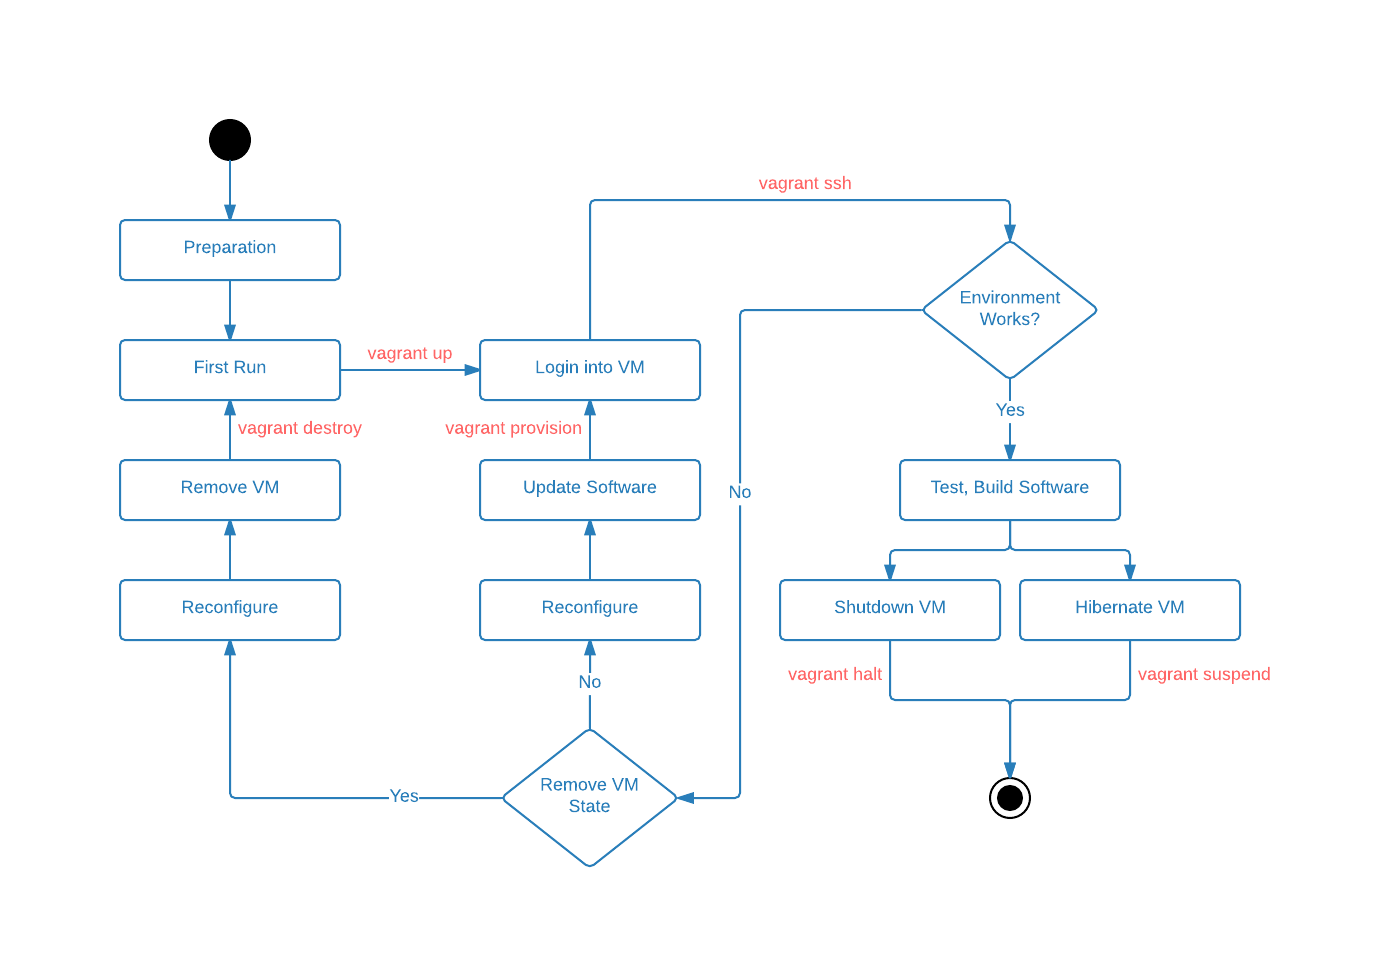
\includegraphics[scale=0.65]{imagenes/vagrant-workflow.png}
	\caption{Flujo de trabajo de Vagrant.\cite{image-vagrant} \label{fig:figura6}}
\end{figure}


\subsection{Ansible}

Ansible\cite{ansible} es un software que se ha diseñado explícitamente para automatizar acciones y
conseguir una mayor productividad. De esta manera, se libera al equipo de tareas costosas
y que siempre siguen el mismo proceso.\\

Ansible está categorizado bajo el nombre de \textbf{herramienta de orquestación} debido a 
las funciones que realiza. Se encarga de manejar nodos a través de \textit{SSH} habiendo recibido
una entrada por parte del usuario. De esta manera, se le proporciona una entrada muy sencilla
y comprensible para la lectura del ser humano, que posteriormente es analizada y transformada
en una serie de tareas hacia los nodos, consiguiendo quedar completamente configurados de una
manera eficiente.\\

\begin{figure}[H]
	\centering
	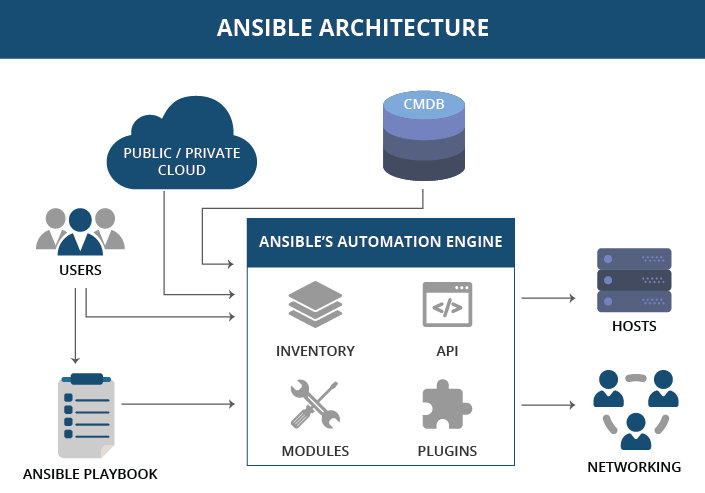
\includegraphics[scale=0.45]{imagenes/ansible.png}
	\caption{Arquitectura de Ansible.\cite{image-ansible} \label{fig:figura7}}
\end{figure}

Como podemos comprobar en la figura anterior, Ansible se encarga de realizar todas las acciones
necesarias para que nuestro software esté listo para desplegarse \textbf{de manera automática}.
De este modo, se conseguirá una mejora significable en el tiempo de despliegue de una aplicación
además de en la gestión del tiempo de los desarrolladores.\\

Es la herramienta de automatización de código libre más potente actualmente y esto es reflejado
en las estadísticas de GitHub del proyecto. Además, la comunidad está implicada muy directamente
en el desarrollo de esta herramienta ya que cuenta con más de 2.400 personas que han desarrollado
uno o varios módulos para mejorarla.

\subsection{Carbone}
Carbone\cite{carbone} no es una herramienta más en el desarrollo de la aplicación. Su uso deriva de la inexistencia de un sistema de gestión documental libre que ofrezca la posibilidad de administrar, rellenar y almacenar las plantillas necesarias. Por tanto, utilizando \textit{Carbone} como base se ha realizado un sistema de gestión documental a medida para este proyecto, consiguiendo todas las funcionalidades nesearias para el correcto funcionamiento de la aplicación y de una manera libre y gratuita.\\

Carbone es una herramienta que permite la inyección de datos en documentos provenientes tanto de LibreOffice como de Microsoft Office, aceptando por tanto la gran mayoría de documentos de texto. De hecho, funciona con todos los documentos basados en el formato \textit{XML}, por lo que su alcance no solo se remite a los programas y formatos previamente mencionados.\\

Esta herramienta es la que ha conseguido que se puedan generar documentos de texto rellenos con los datos adquiridos a través de la aplicación web. Su funcionamiento es simple.\\

\begin{enumerate}
	\item \textbf{Lee una plantilla adaptada.} Le indicamos donde se encuentra la plantilla sobre la que queremos escribir. 
	\item \textbf{Analiza el documento.} Analiza completamente la plantilla en busca de los marcadores \{ y \}.  
	\item \textbf{Recibe los datos en formato \textit{JSON}.} Nuestra aplicación le proporciona los datos que queremos inyectar en el documento con formato \textit{JSON}.  
	\item \textbf{Inyecta los datos.} Realiza una sustitución del contenido de nuestros datos en los marcadores que ha encontrado previamente sobre el documento.
	\item \textbf{Escribe en el fichero destino.} Una vez realiza las sustituciones, procede a escribir el documento resultante en el disco. 
\end{enumerate}

Además de realizar sustituciones, esta herramienta se puede utilizar para dar formato a los datos, repetir porciones del documento como pueden ser filas de una tabla, añadir lógica a la inyección de los datos... Para ayudar a la comprensión, se presenta el siguiente caso de uso real como ejemplo:\\

\textit{Nuestra aplicación genera el siguiente archivo en formato JSON después de que un agente haya rellenado los datos de un formulario.}

\begin{figure}[H]
	\centering
	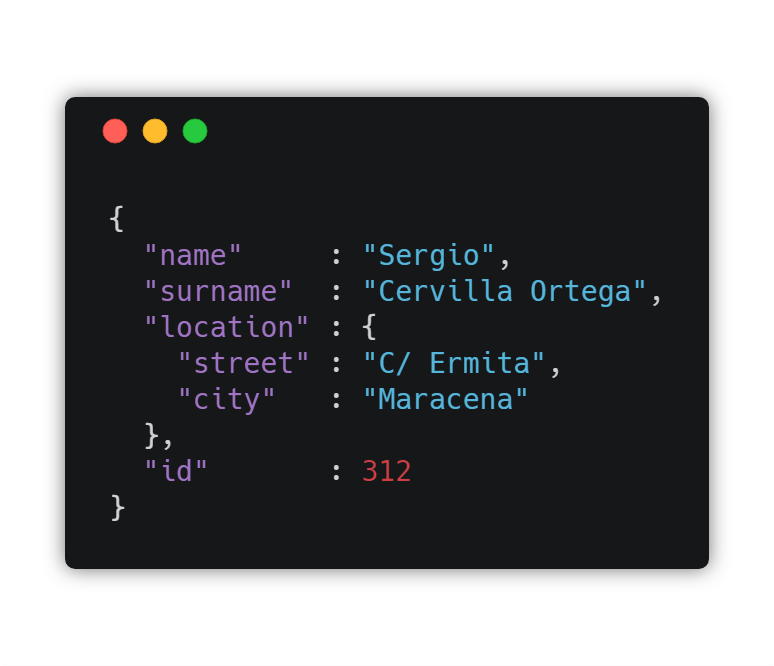
\includegraphics[scale=0.4]{imagenes/json-carbone.png}
	\caption{JSON generado por la aplicación \label{fig:figura10}}
\end{figure}
\newpage

\textit{Una vez disponemos del archivo JSON con los datos, lo utilizamos junto a la plantilla en la que queremos escribir el contenido de dicho archivo, que tendrá el siguiente formato: }

\begin{figure}[H]
	\centering
	\resizebox{\textwidth}{!}{%
	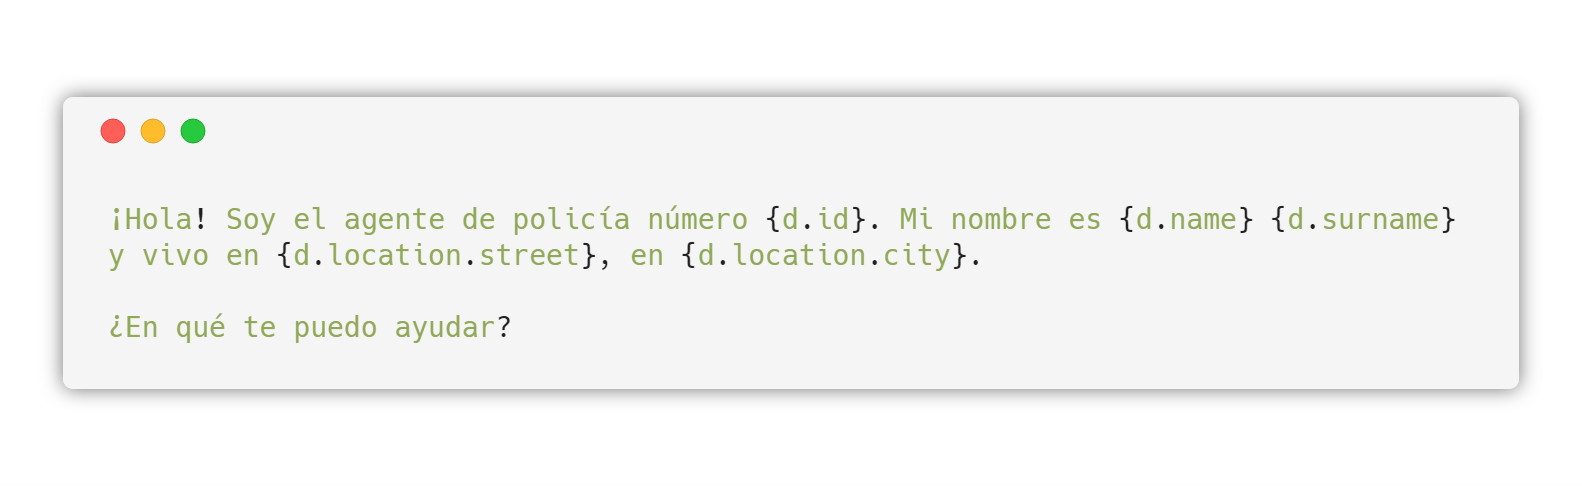
\includegraphics{imagenes/carbone-template.png}}
	\caption{Plantilla sobre la que inyectar los datos. \label{fig:figura11}}
\end{figure}

\textit{Una vez procesados los datos sobre la plantilla, obtendremos el siguiente documento:}
\begin{figure}[H]
	\centering
	\resizebox{\textwidth}{!}{%
		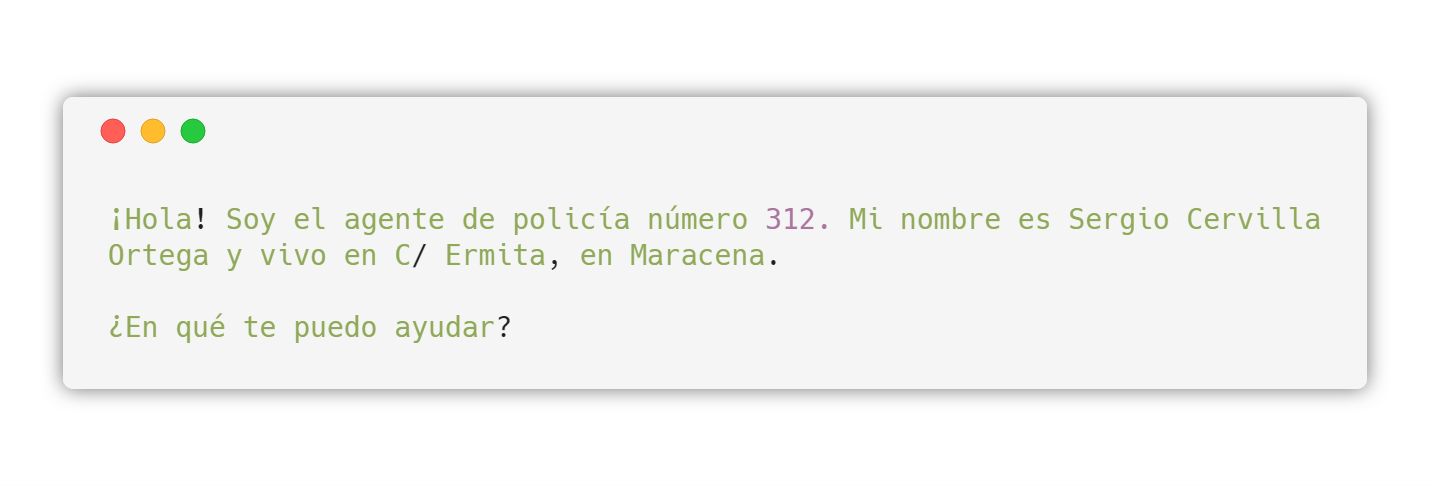
\includegraphics{imagenes/carbone-result.png}}
	\caption{Resultado final tras usar Carbone. \label{fig:figura12}}
\end{figure}

Con este ejemplo, queda claro el uso que tiene en \textbf{Chief} y lo sencillo que es de utilizar esta herramienta para generar documentos de texto rellenos mediante inyección de datos.

	
